\documentclass{article}
\usepackage{xeCJK}
\setCJKmainfont{FandolSong}
\setCJKmonofont{Noto Sans Mono CJK SC}
\usepackage{amsmath}
\usepackage{amsthm}
\usepackage{amssymb}
\usepackage[noend]{algpseudocode}
\usepackage[margin=1in]{geometry}
\usepackage{float}
\usepackage{hyperref}
\setlength{\parindent}{0pt}
\renewcommand{\thesection}{\arabic{section}}
\newcommand{\problem}{\refstepcounter{section}\section*{Problem \thesection}}
\renewcommand{\thesubsection}{(\alph{subsection})}
\newcommand{\subproblem}[1][]{\refstepcounter{subsection}\paragraph{\thesubsection{}#1}\hspace{0pt}}
\newcommand{\tightsubproblem}[1][]{\refstepcounter{subsection}\textbf{\thesubsection#1\hspace{2ex}}}
\newcommand{\ta}[1]{\textsc{#1}}
\newcommand{\admit}{\hfill$\square$}
\newtheorem{lem}{Lemma}
\newtheorem{thm}{Thm}[section]
\newtheorem{co}{Co}[thm]
\algrenewcommand\algorithmiccomment[1]{\hfill// #1}
\renewcommand\qedsymbol{$\blacksquare$}
\newenvironment{algo}[3][1]{

\vspace{1em}
\begin{minipage}{\linewidth}
\ta{#2}($#3$)
\begin{algorithmic}[#1]
}{\end{algorithmic}\end{minipage}}

\author{221900006 耿天成}
\date{\today}
\usepackage{tikz}
\usetikzlibrary{arrows.meta}

\title{ALG Problem Set 10}

\begin{document}
\maketitle

\problem %1
\subproblem %a
Traversing the graph to the first leaf node in a DFS tree, given by the following theorem, reaches a non-key vertex.
\begin{thm} Let $T$ be a spanning tree of $G$. If $u$ is a leaf node of $T$, then $u$ is not a key vertex of $G$. \end{thm}
\begin{proof}
Assume to the contrary that $u$ is a key vertex of $G$, the deletion of $u$ disconnects $G$. Then it also disconnects $T$, but $T-u$ is a tree. Therefore, $u$ is not a key vertex of $G$.
\end{proof}
\begin{algorithmic}[1]
\State $u = V[1]$
\While{$u.vis = \it False$}
    \State $u.vis = \it True$
    \For{each $v$ in $G.Adj[u]$}
        \If{$u.vis = \it False$}
            \State $u=v$
            \State \textbf{break}
        \EndIf
    \EndFor
\EndWhile
\State \Return $u$
\end{algorithmic}
\subproblem %b
$T - u$ is a spanning tree of $G - u$. Let the deletion order be the post-traversal order of $T$. In each deletion, a leaf node of $T$, aka a non-key vertex of $G$, is deleted, and the remaining tree is a spanning tree of the remaining graph. By induction, the post-traversal order of the DFS tree is a valid deletion order.\\[1em]
\ta{DFS1}$(G,u,result)$
\begin{algorithmic}[1]
\State $u.vis = \it True$
\For{each $v$ in $G.Adj[u]$}
    \If{$v.vis = \it False$}
        \ta{DFS1}$(G, v)$)
    \EndIf
\EndFor
\State \ta{Append}$(result, u)$
\end{algorithmic}\vspace{1em}
\ta{DeletionOrder}$(G)$
\begin{algorithmic}[1]
\State \Return $result$ in \ta{DFS1}$(G, G.V[1], [\,])$
\end{algorithmic}
\problem %2
\subproblem %a
% (x1 ∨ x2) ∧ (x1 ∨ x3) ∧ (x1 ∨ x2) ∧ (x3 ∨ x4) ∧ (x1 ∨ x4)
    $G_I$ where $I=(x_1 \vee \overline{x_2}) \wedge (\overline{x_1} \vee \overline{x_3}) \wedge (x_1 \vee x_2) \wedge (\overline{x_3} \vee x_4) \wedge (\overline{x_1} \vee x_4)$: \\[1em]
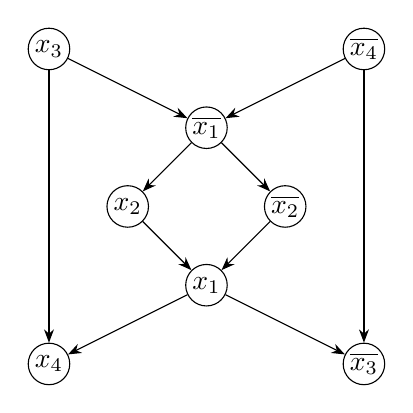
\begin{tikzpicture}[
    every node/.style={circle, draw, minimum size=15pt, inner sep=0pt},
    >={Stealth} % 箭头样式
]
    \node (n1) at (0, 0) {$x_4$};
    \node (n0) at (2, 1) {$x_1$};
    \node (n4) at (4, 0) {$\overline{x_3}$};
    \node (n2) at (1, 2) {$x_2$};
    \node (n6) at (3, 2) {$\overline{x_2}$};
    \node (n3) at (0, 4) {$x_3$};
    \node (n7) at (4, 4) {$\overline{x_4}$};
    \node (n5) at (2, 3) {$\overline{x_1}$};
    \draw[->] (n0) -- (n1);
    \draw[->] (n2) -- (n0);
    \draw[->] (n3) -- (n1);
    \draw[->] (n0) -- (n4);
    \draw[->] (n5) -- (n6);
    \draw[->] (n5) -- (n2);
    \draw[->] (n6) -- (n0);
    \draw[->] (n3) -- (n5);
    \draw[->] (n7) -- (n4);
    \draw[->] (n7) -- (n5);
\end{tikzpicture} \\[1em]
Let $f:V\to\{\textit{True},\textit{False}\}$, $f(\overline{x_i})=\neg f(x_i)$. $f(x_1), f(x_2), \cdots, f(x_n)$ be an assignment of $x_1, x_2, \cdots x_n$. \\[1ex]
\tightsubproblem %b
\textit{Proof.} Assume $I$ is satisfiable. Exists $f$, $I(f(x_1), f(x_2), \cdots, f(x_n))=\it True$. Since for each $(u, v)\in E$, clause $\overline{u}\lor v$ or $v\lor\overline{u}$ is in $I$. So $\textit{True}  =\overline{u}\lor v=\neg f(u)\lor f(v)$, $f(u)\rightarrow f(v)$. Because of $x_i$ and $\overline{x_i}$ is in a connected component, $x_i \rightarrow^{*} \overline{x_i}$ and vice versa. Boolean algebra on the paths between $x_i$ and $\overline{x_i}$ gives a contradictory formula $f(x_i)\leftrightarrow\neg f(x_i)$. Therefore, $I$ is unsatisfiable.
\hfill\qedsymbol
\subproblem %c
\label{p2:scc}
\textit{Proof.} Induction on $n$. The base case is $n=0$, nothing to assign. Suppose it is true for all $n'<n$. Choose one $SCC$ that has no outgoing edge. Assign $\it True$ to all $u\in SCC$ and $\it False$ to corresponding $\overline{u}$. Since $\overline{u}$ is not in $SCC$, there is no conflict. For clause involving $u$: $u \lor v$ is satisfied; $\overline{u} \lor v$ gives $(u, v)\in E$, but $u$ has no outgoing edge. Let $I'$ be an instance of 2SAT by removing all clauses involving $u$ in $I$. The SCCs of $G_{I'}$ do not contain both a literal and its negation. By the induction hypothesis, $I'$ is satisfiable. Therefore, $I$ is satisfiable.
\hfill\qedsymbol
\subproblem %d
Run Tarjan's SCC algorithm on $G_I$. In \ref{p2:scc}, we assign $\it True$ to a vertex topologically larger.
If the topological order in the SCC-DAG is larger, the vertex was traversed later and was popped from the stack earlier, resulting in a smaller component number. Therefore, we can assign $\it True$ to the one with the smaller component number in the affirmation-negation pair.
\begin{algorithmic}[1]
\State Build $(V, E)=G_I$ as described
\State $scc=\ta{TarjanSCC}(V, E)$
\For{each variable $x$}
    \If{$scc[x] < scc[\overline{x}]$}
        \State $solution[x] = \it True$
    \ElsIf{$scc[x] > scc[\overline{x}]$}
        \State $solution[x] = \it False$
    \Else
        \State \Return {\it NIL}
    \EndIf
\EndFor
\State \Return $solution$
\end{algorithmic}
Runtime: building $G_I$ takes $O(|V|+|E|)$, and so does $\ta{TarjanSCC}$. The loop takes $O(|V|)$. The algorithm has linear runtime.
\problem %3
\begin{lem}
Let $T$ be a tree and $(u, v)\in T$ be an edge on $T$. Then $T - \{u, v\}$ is a forest having exactly 2 connected components (CC) $C_u$ and $C_v$, where $u\in C_u$ and $v \in C_v$.
\end{lem}
\begin{proof}
Given by the property of tree.
\end{proof}

\subproblem True. Formally, let $T$ be an MST of $G$ with weight function $w$, $(u, v)\in T$. Then there exists some cut $(S, V-S)$ of $G$ so that $(u, v)$ is a light edge cross $(S, V-S)$.
\begin{proof}
Let $C_u, C_v$ be the 2 CCs of $T - \{(u, v)\}$. If $(u, v)$ is not a light edge cross $(C_u, C_v)$. Suppose $(x, y)$ is crossing $(C_u, C_v)$ and $w(x, y) < w(u, v)$, then $T - \{(u, v)\} \cup \{(x, y)\}$ is a spanning tree weight smaller that $T$. Contradictory.
\end{proof}
\subproblem True.
\begin{thm} \label{thm:unique} A graph has a unique minimum spanning tree if, for every cut of the graph, there is a unique light edge crossing the cut. \cite{23.1-6} \end{thm}
\begin{proof} \cite{23.1-6sol}
Assume to the contrary that the graph has 2 different MSTs, $T$ and $T'$. There exists at least one edge $(u, v) \in T$ and $(u,v)\notin T'$. $(u, v)$ splits $T$ into into $C_u$ and $C_v$. By reasoning in \textbf{(a)}, $(u, v)$ is the light edge cross $(C_u,C_v)$. There is at least one edge $f$ cross $(C_u, C_v)$ on the path from $u$ to $v$ for $T'$. $w(f) > w(u, v)$. So $w(T'-\{(u, v)\}\cup f)<w(T')$, which contradicts that $T'$ is an MST.
\end{proof}
\subproblem False. $w(2,3)=w(2,4)$, but MST $\{(1,2),(1,3),(3,4)\}$ is unique. \\
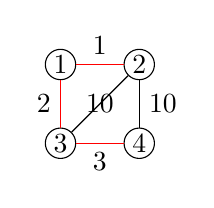
\begin{tikzpicture}
    \node[circle, draw, inner sep=1pt] (3) at (0, 0) {3};
    \node[circle, draw, inner sep=1pt] (1) at (0, 1) {1};
    \node[circle, draw, inner sep=1pt] (2) at (1, 1) {2};
    \node[circle, draw, inner sep=1pt] (4) at (1, 0) {4};
    \draw[-] (1) -- (3) node[midway, left] {2};
    \draw[-] (1) -- (2) node[midway, above] {1};
    \draw[-] (2) -- (3) node[midway] {10};
    \draw[-] (3) -- (4) node[midway, below] {3};
    \draw[-] (2) -- (4) node[midway, right] {10};
    \draw[-, color=red] (1) -- (2);
    \draw[-, color=red] (1) -- (3);
    \draw[-, color=red] (3) -- (4);
\end{tikzpicture}
\problem
Note: it is required to add a precondition that $|V|\le |E|$ \cite{23-1}, to ensure the existence of a second-best minimum spanning tree (SMST).
\subproblem %a
MST is unique: apply theorem \ref{thm:unique}. We need to show that for every cut, there is a unique light edge. It is true because each edge has unique weight.

The following graph has $w(\textit{MST})=7, w(\textit{SMST})=8$. It has 2 SMST $\{(1,2),(2,3),(3,4)\}$ and $\{(1,3),(2,3),(2,4)\}$. \\[1ex]
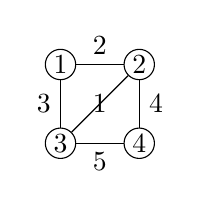
\begin{tikzpicture}
    \node[circle, draw, inner sep=1pt] (3) at (0, 0) {3};
    \node[circle, draw, inner sep=1pt] (1) at (0, 1) {1};
    \node[circle, draw, inner sep=1pt] (2) at (1, 1) {2};
    \node[circle, draw, inner sep=1pt] (4) at (1, 0) {4};
    \draw[-] (1) -- (3) node[midway, left] {3};
    \draw[-] (1) -- (2) node[midway, above] {2};
    \draw[-] (2) -- (3) node[midway] {1};
    \draw[-] (3) -- (4) node[midway, below] {5};
    \draw[-] (2) -- (4) node[midway, right] {4};
\end{tikzpicture} \\[1em]
\tightsubproblem \label{thm:cycle} \textit{Proof.}
When $|V| \le |E|$, suppose $A$ is an SMST of $G$. Choose one edge $(x, y)$ from $A \setminus T$.
Let $T_{xy}$ denotes the simple path between $x$ and $y$ on $T$. Let $(u, v)$ be the heaviest edge on $T_{xy}$. We will show that $T'=T - \{(u, v)\} \cup \{(x, y)\}$ is an SMST.
It is required to show that $w(T')\le w(A)$.
This is equivalent to $w(T)\le w(A) - w(x, y) + w(u, v)$. Let $C_x, C_y$ be the 2 CCs of $A - \{(x, y)\}$. There is at least one edge $f$ on $T_{xy}$ across $(C_x, C_y)$, and $w(f) \le w(u, v)$.
Since $A - \{(x, y)\} \cup \{f\}$ is a spanning tree of $G$, we have $w(T) \le w(A) - w(x, y) + w(f) \le w(A) - w(x, y) + w(u, v)$.
\hfill\qedsymbol
\subproblem For each $u \in V$, we compute $f(v) = max[u, v]$ during a DFS rooted at $u$.\\[1em]
\ta{DFS2}$(Adj, w, u, max)$
\begin{algorithmic}[1]
\State $u.vis = \it True$
\For{each $v$ in $Adj[u]$}
    \If{$v.vis = \it False$}
        \State $v.vis = \it True$
        \If{$max[u] = \textit{NIL} \lor w(u, v) > w(max[u])$}
            \State $max[v] = (u, v)$
        \EndIf
        \State \ta{DFS2}$(Adj, w, v, max)$
    \EndIf
\EndFor
\end{algorithmic}\vspace{1em}
\ta{MaxWeightEdges}$(G, T, w)$
\begin{algorithmic}[1]
\State Initialize $max[G.V][G.V]$ with $\it NIL$
\For{each $(u, v)$ in $T$}
\State $\ta{Append}(Adj[u], v)$
\State $\ta{Append}(Adj[v], u)$
\EndFor
\For{each $u$ in $V$}
\State For all $x$ in $V$, $x.vis = \it False$
\State \ta{DFS2}$(Adj, w, u, max[u])$
\EndFor
\State \Return $max$
\end{algorithmic}\vspace{1em}
The running time for each $\ta{DFS2}$ is $O(|V|)$. Total running time is $O(|V|^2)$.
\subproblem First, we compute an MST $T$. In \ref{thm:cycle} we prove that there exists some edge $(x, y)\in E - T$, and $(u, v)\in T$ be the edge of maximum weight on the path between $x$ and $y$ on $T$ , such that $T - \{(u, v)\}\cup \{(x, y)\}$ is an SMST. The algorithm then tries every $(x, y)$, obtaining a subset of $\mathcal{T}-\{T\}$. At least one SMST is in the subset.
So a spanning tree in the subset of minimum weight is an SMST. \\[1em]
\ta{SecondMST}$(G, w)$
\begin{algorithmic}[1]
\State $T = \ta{Prim}(G, w)$
\State $max = \ta{MaxWeightEdges}(G, T, w)$
\For{each $(u, v)$ in $T$}
    \State $(u, v).tree = \it True$
\EndFor
\State $e = \it NIL$
\For{each $e'$ in $G.E$}
    \If{$e'.tree=\it False$}
        \If{$e = \textit{NIL}\lor w(e) - w(max[e]) > w(e') - w(max[e'])$}
            \State $e = e'$
        \EndIf
    \EndIf
\EndFor
\State \Return $T + e - max[e]$
\end{algorithmic}\vspace{1em}
Running time analysis: \\[1em]
\begin{tabular}{l|c} \hline
Line(s) & Time \\\hline
1 & $T(\ta{Prim})$ \\
2 & $O(|V|^2)$ \\
3-4 & $O(|V|)$ \\
7 & $O(1)$ \\
8-9 & $O(|E|)$ \\
10 & $O(|V|)$ \\\hline
Total & $O(\ta{Prim} + |V|^2)$ \\\hline
\end{tabular} \\[1em]
The running time of $\ta{Prim}$, in the textbook, is related to the choice of priority queue. If we implement it with brute force, where $\ta{ExtractMin}$ takes O($|V|$) and $\ta{DecreaseKey}$ takes $O(1)$. Then $T(Prim) = O(|V|^2+E) = O(|V|^2)$.
The total running time is $O(|V|^2)$, as specified.
\problem %5
\begin{algorithmic}[1]
\State sort $(L, R)$ in ascending order by $L$
\State $i = 2, j = 1$
\State $C = \{(L[1], R[1])\}$
\While{$i \le n$}
    \State{$t=j$}
    \While{$i\le n$ and $L[i]\le R[j]$}
        \If{$R[t]<R[i]$}
            \State $t=i$
        \EndIf
        \State $i=i+1$
    \EndWhile
    \If{$t\neq j$}
        \State $\ta{Insert}(C, (L[t], R[t]))$
        \State $j=t$
    \ElsIf{$i \le n$}
        \State $\ta{Insert}(C, (L[i], R[i]))$
        \State $j=i$
        \State $i=i+1$
    \EndIf
\EndWhile
\State \Return C
\end{algorithmic}\vspace{1em}
The running time is $O(n)$.
For each iteration of the outer loop from line 4 to line 16, assume $i$ increases by $\Delta_i$. And assume in the inner loop from line 6 to line 9, $i$ increases by $\delta_i$.
\begin{itemize}
    \item If $\delta_i=0$, then $t=j$ at line 10. $\Delta_i=1$ by line 16. The iteration takes $O(1)=O(\Delta_i)$ time.
    \item If $\delta_i>0$, the iteration takes $O(\delta_i)+O(1)=O(\Delta_i)$ time.
\end{itemize}
The running time of each iteration of the outer loop is $O(\Delta_i)$. So the total running time of the outer loop is $\sum O(\Delta_i)=O(n)$.
\paragraph{Correctness}
\begin{thm}
    At the start of each iteration of the outer loop, $C$ is a cover of $X_i = \{(L_k, R_k) \mid k < i \}$, $R_j = \max\{R_k \mid k < i\}$, and $C$ is a subset of some smallest cover of $X$.
\end{thm}
\begin{proof}
    Induction on iterations. The base case is when $i=2, j=1, C=X_2=\{(L_1, R_1)\}$. $C$ is the smallest cover of $X_2$ and $R_1=\max\{R_1\}$. Since $(L_1, R_1)$ is the only interval that covers point $L_1$, it should be included in any cover of $X$. So $C$ is a subset of some smallest cover of $X$. \\
    Suppose at the start of outer iteration $i_{5}$, the invariant holds.
    After the inner loop,
    $$\forall k<i_{10}.(L_k\le R_j),\ R_t=\max\{R_k\mid k<i_{10}\},\text{ and}\ i_{10}=n+1\lor R_{i_{10}} > R_j$$
    Let $k$ be index that $L_k \le R_j < R_k$. $S$ be the set of $k$. Then $i_5\le k < i_{10}$.
    \begin{enumerate}
        \item If $S=\emptyset$, then $t=j$. $C$ covers $\{(L_k, R_k)\mid k<i_{10}\}$. If $i_{10}\le n$, same as the base case, $i_{10}$ is included in the smallest cover of $X$. The invariant holds for the next iteration where $i=i_{10}+1, j=i$.
        \item If $S\neq\emptyset$, then $t\neq j$. We need to show that $C\cup \{(L_t, R_t)\}$ is a subset of some smallest cover of $X$. Suppose $C\subseteq C_{opt}$, $C_{opt}$ is a smallest cover of $X$. If $(L_t, R_t)\in C_{opt}$, we are done.
        If $(L_t, R_t)\notin C_{opt}$, choose one interval $I$ in $C_{opt}\cap S$. $C\cup (L_t, R_t)$ covers $C\cup I$. So $C\subseteq C_{opt}-I\cup (L_t, R_t)$ is a subset of some smallest cover of $X$. The invariant holds for the next iteration $i=i_{10}, j=t$.
    \end{enumerate}
\end{proof}
\paragraph{Termination:} when the loop ends, $i=n+1$ and $C$ is a smallest cover of $X_{n+1}=X$.
\problem %6
\subproblem %a
\begin{enumerate}
    \item Incorrect. \{(1,4),(2,3),(3,4)\}. {\it Opt} = \{(2,3),(3,4)\}, but the strategy selects \{(1,4)\}.
    \item Correct. \label{stgy:2} \textit{Proof.} Map each activity $(l, r)$ to $(-r, -l)$. The optimal selection on mapped intervals is also an optimal selection. Since the strategy ``choose activity ends first'' is correct. The reflection strategy ``choose activity starts last'' is correct. \hfill\qedsymbol
    \item Incorrect. \{(1,4),(3,5),(4,7)\}. {\it Opt} = \{(1,4),(4,7)\}, but the strategy selects \{(3,5)\}.
    \item Incorrect. An counterexample with 11 activities: \begin{align*}\{(1,2),(2,4),(4,6),(6,7),(3,5),(1,3),(1,3),(1,3),(5,7),(5,7),(5,7)\}\end{align*}
    {\it Opt} = \{(1,2),(2,4),(4,6),(6,7)\}. But the strategy will first choose $(3,5)$, which has 2 conflicts, and gives a size 3 selection.
    \item Correct. For any optimal selection $S$, if any $x\in S$ completely contains another activity $y$, $S - \{x\} \cup \{y\}$ is an optimal selection. After discarding useless activities, the activity that ends last must start last (if it starts earlier than $y$, then it contains $y$). The strategy is correct by the correctness of strategy \ref{stgy:2}.
\end{enumerate}
\subproblem %b
None of the strategies is correct. The strategies don't consider weight. Suppose the activities are $\{(1, 3), (2, 4)\}$. If the strategy outputs $\{(1, 3)\}$, then let $w(1, 3) < w(2, 4)$ and it fails. Otherwise let $w(1, 3) > w(2, 4)$ and it fails.

\begin{thebibliography}{9}
\bibitem{23.1-6} (CLRS) Thomas H. Cormen, Charles E. Leiserson, Ronald L. Rivest, and Clifford Stein. 2009. Introduction to Algorithms, Third Edition (3rd. ed.). The MIT Press. Page 630. Exercise 23.1-6.
\bibitem{23.1-6sol} url: \url{https://walkccc.me/CLRS/Chap23/23.1/#231-6}
\bibitem{23-1} CLRS. Page 638. Problem 23-1.
\end{thebibliography}
\end{document}